\subsubsection{Decomposi\c c\~ao STL}\label{subsubsec:stl}

A decomposição sazonal e de tendência utilizando o procedimento de Loess (STL) é uma técnica amplamente utilizada para decompor séries temporais em seus componentes sazonais, de tendência e restantes. De acordo com \citeonline{Theodosiou20111178}, o método STL realiza a decomposição aditiva dos dados por meio de uma sequência de aplicações do Loess mais suave, onde regressões polinomiais ponderadas localmente são aplicadas em cada ponto do conjunto de dados, tendo como variáveis explicativas os valores mais próximos do ponto cuja resposta está sendo estimada.

A decomposição STL é especialmente útil para identificar e isolar padrões sazonais e de tendência presentes nas séries temporais. Ela permite a separação dos componentes sazonais, que ocorrem em intervalos regulares ao longo do tempo, da componente de tendência, que indica a direção geral dos dados ao longo do tempo. A decomposição também resulta em uma componente restante, que representa a variação não explicada pelos componentes sazonais e de tendência.

Ao aplicar a decomposição STL, a série temporal pode ser expressa como a soma dos componentes sazonais, de tendência e restantes. Essa técnica é útil para análise e modelagem de séries temporais, pois proporciona uma compreensão mais clara dos padrões de variação presentes nos dados.

A decomposição STL é formalmente definida como:

\begin{eqnarray}
	y_t=f\left(S_t, T_t, R_t\right)&=&\left\{\begin{array}{l}
		y_t=S_t+T_t+R_t \quad \text { aditivo } \\
		y_t=S_t T_t R_t \quad \text { multiplicativo }
	\end{array}\right. \label{eq:stl}
\end{eqnarray}

\begin{figure}[H]
	\centering
	\caption{Decomposição STL aditiva dos dados coletados}
	\label{fig:stl-aditiva}
	\includegraphics[width=0.9\linewidth]{"Resultados/Figuras/STL aditiva"}
	
	Fonte: Elaboração própria a partir de dados da SANEPAR (2018 a 2020)
\end{figure}


\begin{figure}[H]
	\centering
	\caption{Decomposição STL multiplicativa dos dados coletados}
	\label{fig:stl}
	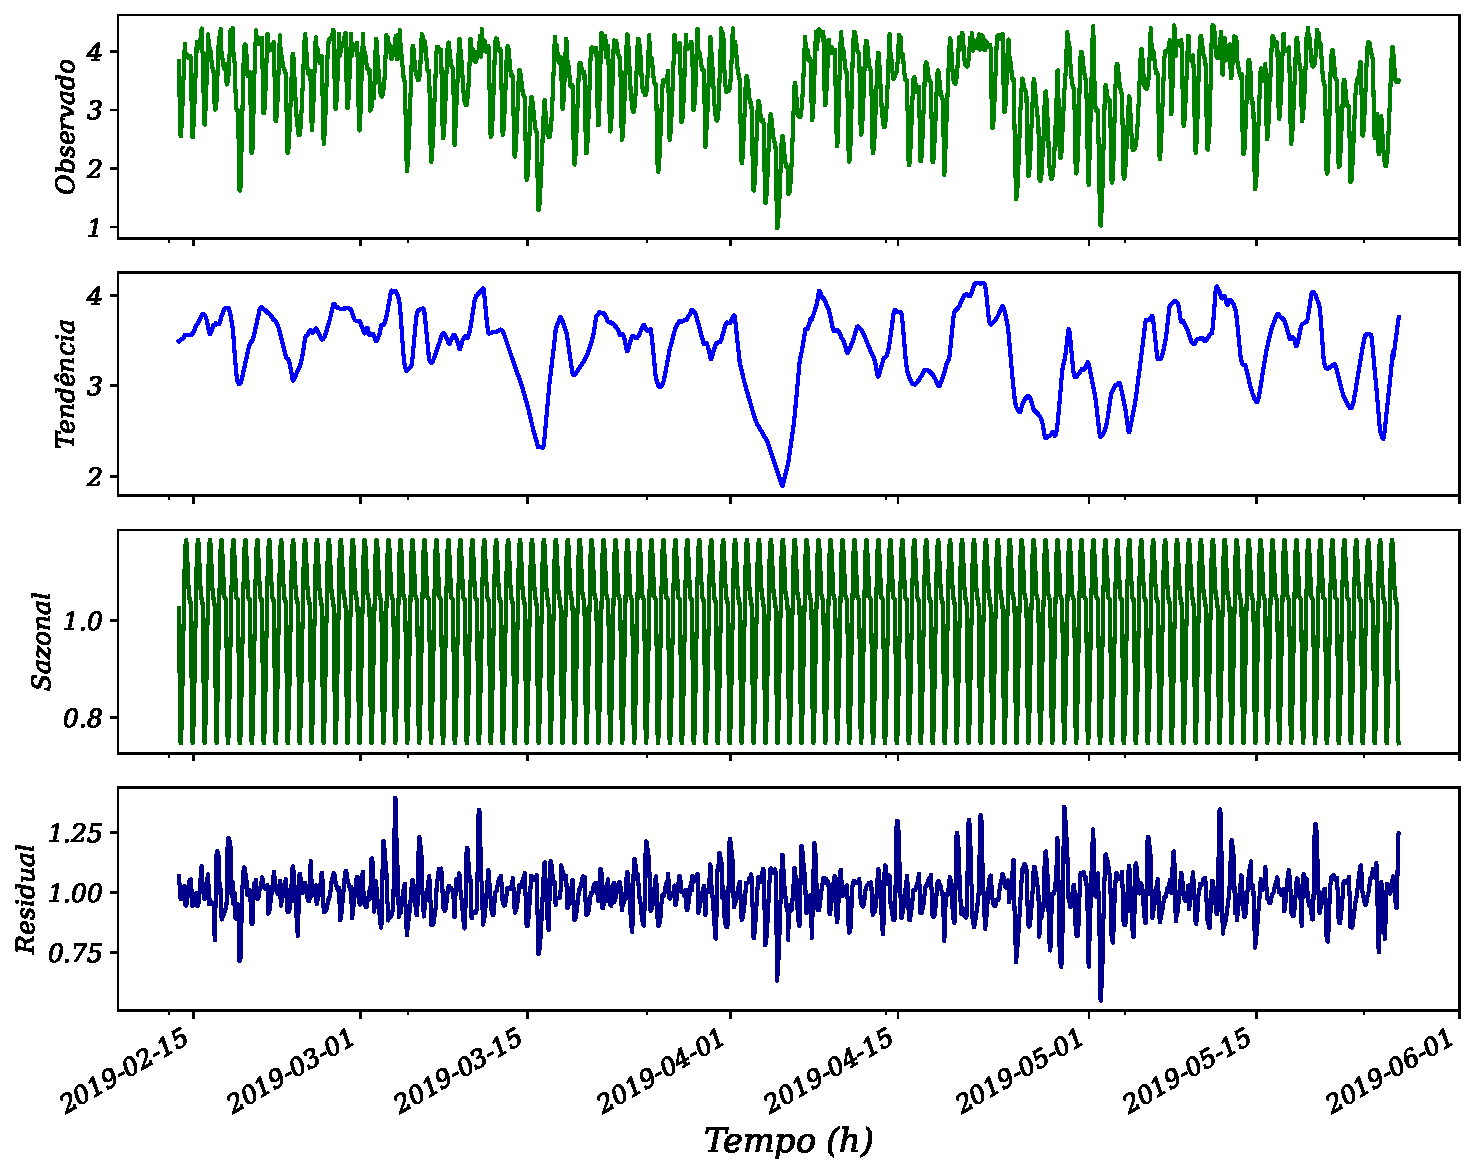
\includegraphics[width=0.9\linewidth]{Resultados/Figuras/STL}
	
	Fonte: Elaboração própria a partir de dados da SANEPAR (2018 a 2020)
\end{figure}

Na resposta à pergunta \ref{q5}\ref{q5:b}, as Figuras \ref{fig:stl-aditiva} e \ref{fig:stl} fornecem informações sobre a presença de tendência, sazonalidade e resíduos na série temporal.

Através da decomposição, é possível analisar se a série apresenta tendência, sazonalidade e resíduos. Ao observar as Figuras \ref{fig:stl-aditiva} e \ref{fig:stl}, é evidente que os dados exibem ambos os padrões. Isso indica que a série é estacionária, como confirmado pelo seguinte teste.

Teste de Dickey-Fuller (DF) Aumentado:
\begin{itemize}
	\item Estatística de teste ADF: $-4.248$
	\item Valor de p: $0.001$
	\item Atrasos utilizados: $21.000$
	\item Observações: $1074.000$
	\item Valor crítico (1\%): $-3.436$
	\item Valor crítico (5\%): $-2.864$
	\item Valor crítico (10\%): $-2.568$
\end{itemize}

Com base na forte evidência contra a hipótese nula, podemos rejeitar a hipótese nula. Isso indica que os dados não possuem raiz unitária e são estacionários em \ref{q5}\ref{q5:c}. Identificar as horas de pico entre 18h e 21h não é uma tarefa fácil. No entanto, ao observar a Figura \ref{fig:hist}, podemos notar um aumento na demanda durante essas horas durante o ano de 2020.
	
	
	\begin{figure}[H]
		\centering
		\caption{Violino no nível do reservatório}
		\label{fig:hist}
		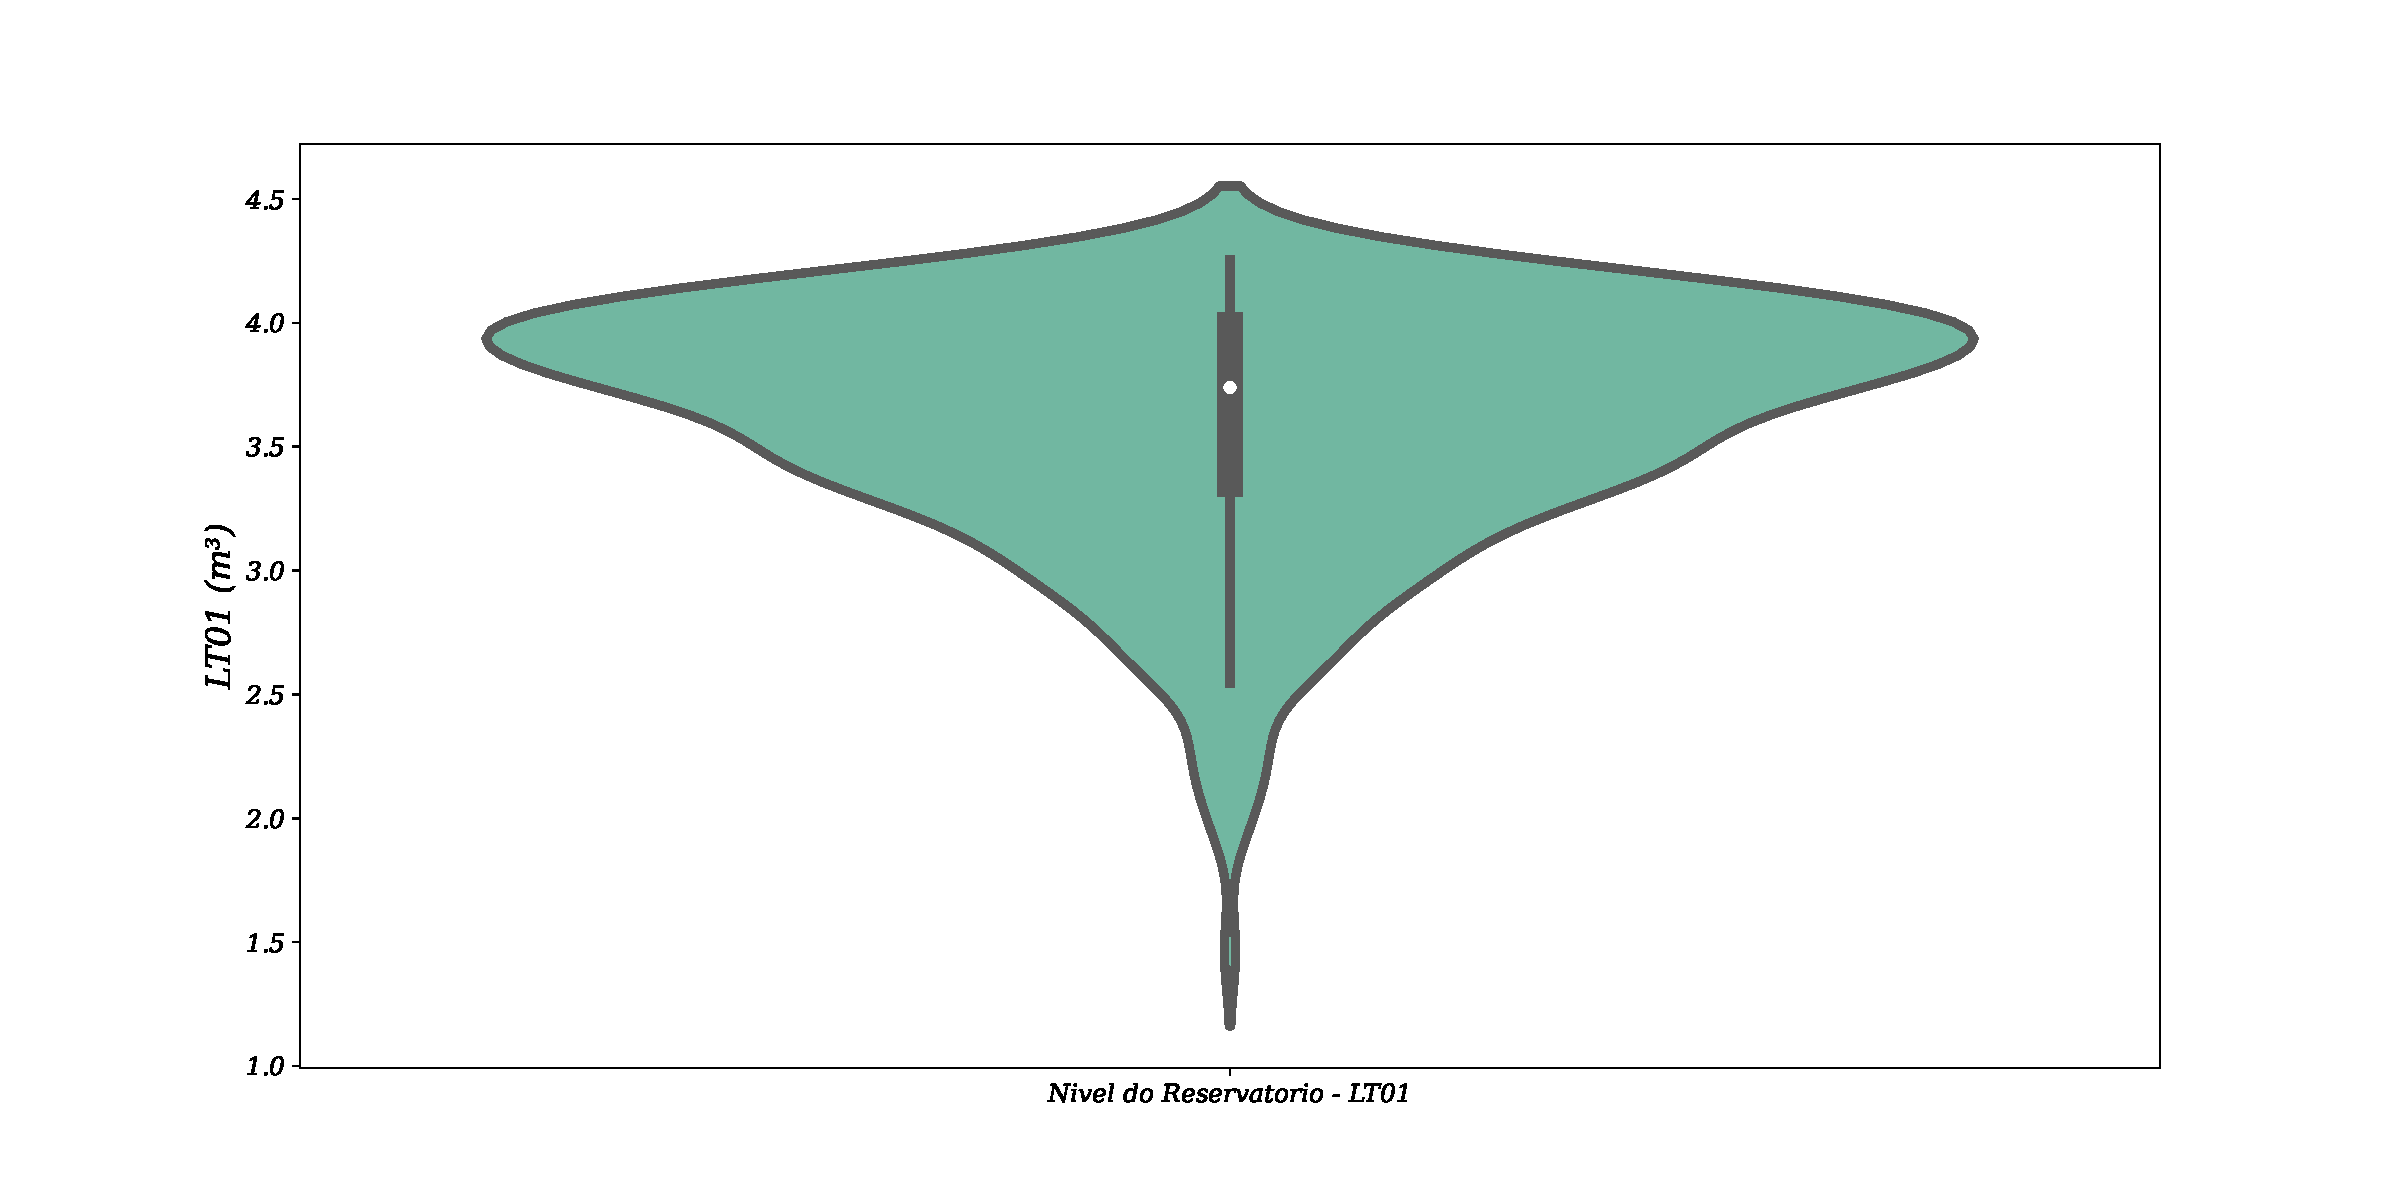
\includegraphics[width=0.9\linewidth]{Resultados/Figuras/viol}
		
		Fonte: Elaboração própria a partir de dados da SANEPAR (2018 a 2020)
	\end{figure}
	
Conforme mencionado na subseção \ref{subsubsec:motivacao}, as anomalias climáticas ocorridas em 2020, especialmente a falta de chuvas, tiveram um impacto significativo nos resultados. Isso contribuiu para as mudanças observadas na demanda de água ao longo desse período.

Com relação à pergunta \ref{q5}\ref{q5:d}, durante as horas de pico, é necessário que o nível do tanque esteja dentro da faixa de $[3.545,4.256] m^3$ para evitar o acionamento das bombas. Manter o nível do tanque dentro dessa faixa permitirá que o sistema opere de forma eficiente, atendendo à demanda sem a necessidade de acionar as bombas.
	
	
	\begin{figure}[H]
		\centering
		\caption{Violino da vazão de recalque}
		\label{fig:ft03}
		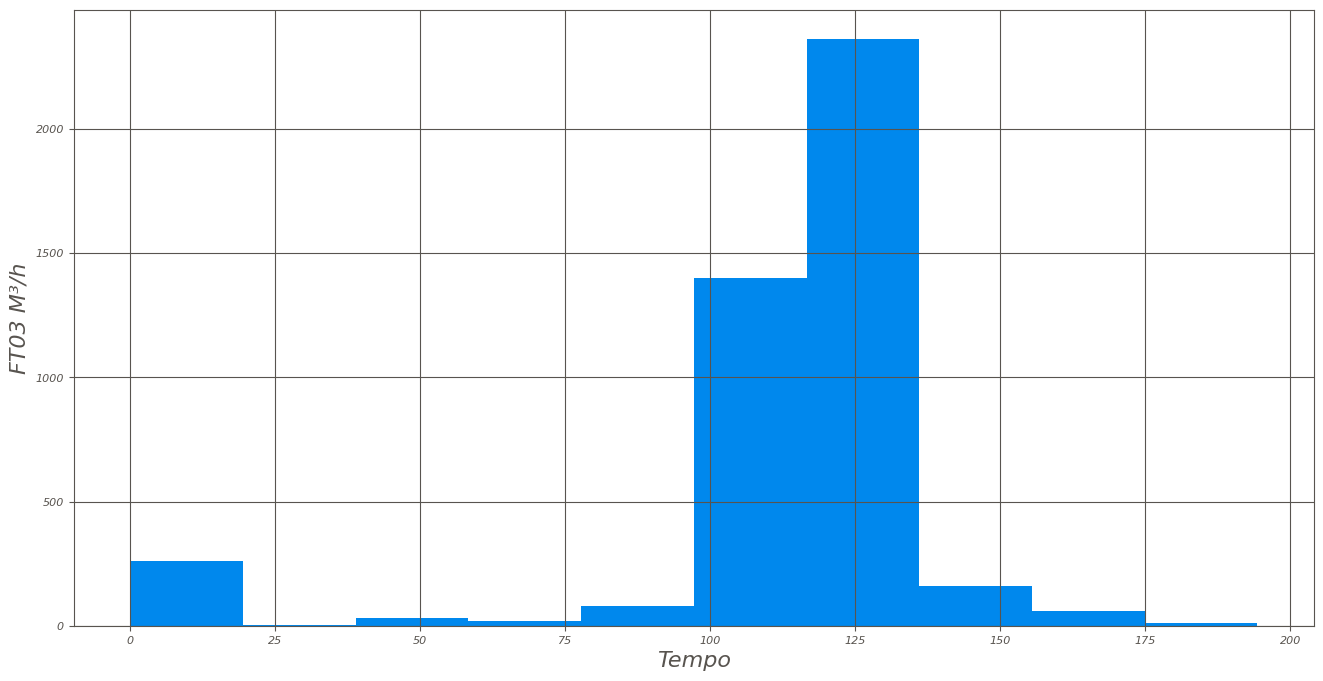
\includegraphics[width=0.9\linewidth]{Resultados/Figuras/ft03}
		
		Fonte: Elaboração própria a partir de dados da SANEPAR (2018 a 2020)
	\end{figure}
	
Para responder à pergunta \ref{q5}\ref{q5:e}, a Figura \ref{fig:ft03} ilustra como a vazão pode ser afetada pelo nível do tanque. É interessante observar que a vazão de recalque tem um impacto mais significativo no nível do tanque em comparação com as outras vazões. Isso ocorre porque a vazão de recalque está associada à injeção de água diretamente no tanque por meio da bomba localizada próxima à base do tanque. Por outro lado, as demais vazões apresentam alguns valores ausentes, o que limita sua influência na análise geral.	
	


De acordo com o \citeonline{Reisen2017115}, o teste DF tem as seguintes equações

\begin{eqnarray}
	z_t&=& y_t+\theta \beta_t, \qquad t=1,\ldots, T, \label{eq:df3}\\	
	\hat{\rho}_{\mathrm{DF}}-1&=&\frac{\sum_{t=1}^T z_{t-1} \Delta z_t}{\sum_{t=1}^T z_{t-1}^2} \label{eq:regdf}
\end{eqnarray}

De \eqref{eq:regdf} onde $\Delta z_t=z_t-z_{t-1}$. Sob a hipótese nula $\left(H_0\right)$ : `` $\rho=1$'', as estatísticas do teste DF e suas distribuições limitantes são dadas da seguinte forma:


\begin{eqnarray}
	T\left(\hat{\rho}_{\mathrm{DF}}-1\right)=T \frac{\sum_{t=1}^T z_{t-1} \Delta z_t}{\sum_{t=1}^T z_{t-1}^2}
\end{eqnarray}
e


\begin{eqnarray}
	\hat{\tau}_{\mathrm{DF}}&=&\frac{\hat{\rho}_{\mathrm{DF}}-1}{\hat{\sigma}_{\mathrm{DF}}\left(\sum_{t=1}^T z_{t-1}^2\right)^{-1 / 2}} \label{eq:df}
\end{eqnarray}

De \eqref{eq:df} onde $\hat{\sigma}_{\mathrm{DF}}^2=T^{-1} \sum_{t=1}^T\left(\Delta z_t-\left(\hat{\rho}_{\mathrm{DF}}-1\right) z_{t-1}\right)^2 .$



Suponha que $\left(z_t\right)_{1 \leq t \leq T}$ são dadas por \eqref{eq:df3}, então quando $\rho=1$,


\begin{eqnarray}
	T\left(\hat{\rho}_{\mathrm{DF}}-1\right) \stackrel{d}{\longrightarrow} \frac{W(1)^2-1}{2 \int_0^1 W(r)^2 \mathrm{~d} r}-\left(\frac{\theta}{\sigma}\right)^2 \frac{\pi}{\int_0^1 W(r)^2 \mathrm{~d} r}, \text { como } T \rightarrow \infty \\
	\hat{\tau}_{\mathrm{DF}} \stackrel{d}{\longrightarrow}\left[1+2(\theta / \sigma)^2 \pi\right]^{-1 / 2}\left\{\frac{W(1)^2-1}{2\left(\int_0^1 W(r)^2 \mathrm{~d} r\right)^{1 / 2}}-\frac{(\theta / \sigma)^2 \pi}{\left(\int_0^1 W(r)^2 \mathrm{~d} r\right)^{1 / 2}}\right\} \\
	\quad \operatorname{como} T \rightarrow \infty\label{eq:df2}
\end{eqnarray}

A partir de \eqref{eq:df2}, onde$\stackrel{d}{\longrightarrow}$ denota convergência na distribuição e onde $\{W(r), r \in[0,1]\}$ denota o movimento Browniano padrão.

O ACF (do inglês \textit{Auto-Correlation Function}) é uma medida estatística utilizada para identificar a presença de correlação serial em uma série temporal. Ele calcula a autocorrelação entre os valores da série em diferentes defasagens, ou seja, a correlação entre os valores atuais e os valores passados da série. 

O ACF é útil para analisar a dependência temporal dos dados e identificar padrões de sazonalidade, tendência ou outros efeitos temporais. Através do ACF, é possível avaliar se a série exibe autocorrelação significativa em defasagens específicas, o que pode indicar a presença de não estacionariedade ou estrutura temporal que precisa ser considerada na análise ou modelagem da série temporal.

\begin{figure}[H]
	\centering
	\caption{Autocorrelação e Autocorrelação parcial}
	\label{fig:acf}
	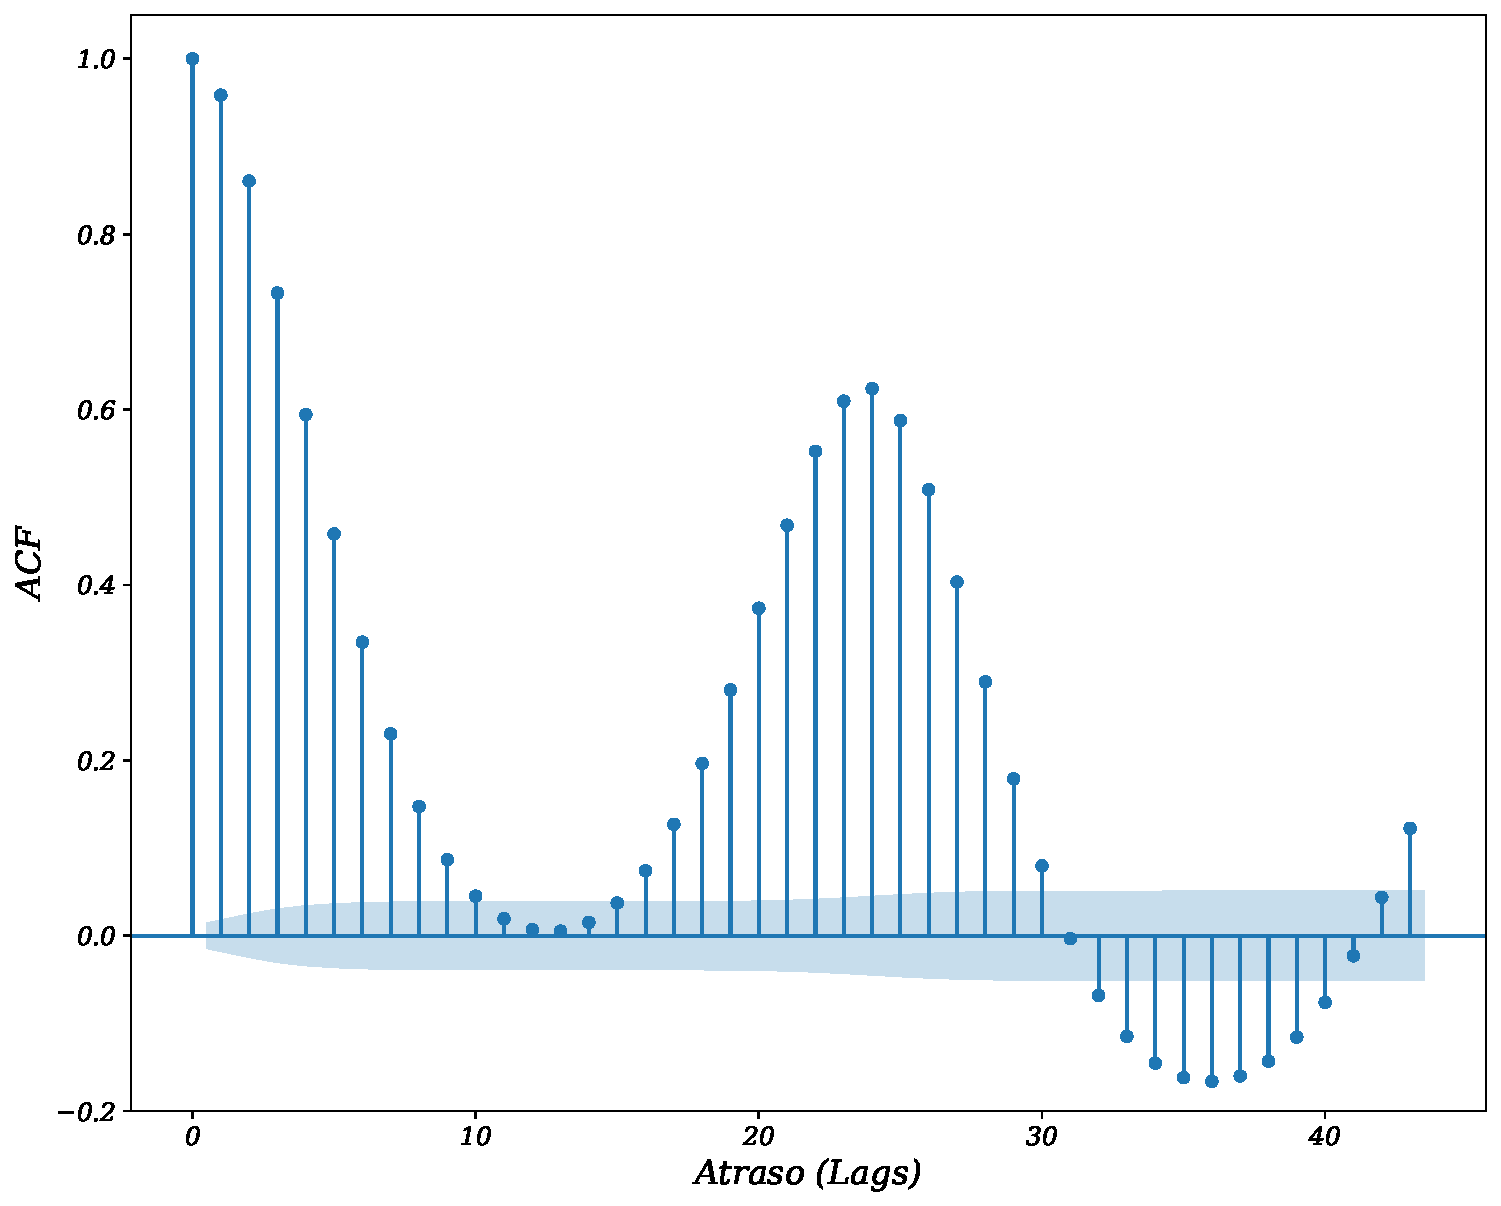
\includegraphics[width=0.9\linewidth]{Resultados/Figuras/acf} 
	
\end{figure}	
\begin{figure}[H]
	\centering
	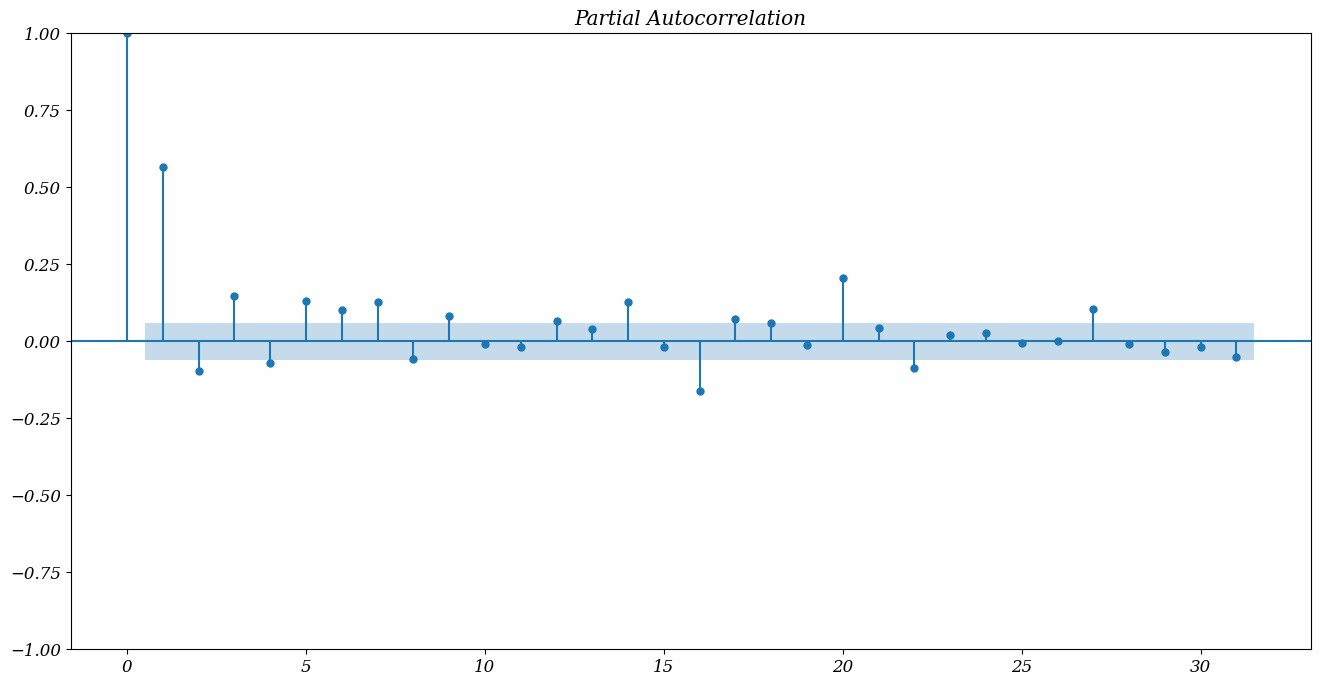
\includegraphics[width=0.9\linewidth]{Resultados/Figuras/pacf}
	
	Fonte: Elaboração própria a partir de dados da SANEPAR (2018 a 2020)
\end{figure}

Na Figura \ref{fig:acf}, é possível observar a diferença entre a autocorrelação e a autocorrelação parcial (PACF). A autocorrelação mede a correlação entre os valores da série temporal em diferentes defasagens, levando em consideração tanto a correlação direta quanto a correlação indireta. Por outro lado, a autocorrelação parcial mede apenas a correlação direta entre os valores, eliminando a influência das defasagens intermediárias.

O intervalo de confiança padrão de 95\% é representado pela marca azul na Figura. As observações que estão fora desse intervalo são consideradas estatisticamente correlacionadas, indicando a presença de padrões ou estrutura na série temporal.

A correlação visualizada na Figura \ref{fig:acf} é fundamental para a interpretação do teste DF. Em uma série de ruído branco, os valores são completamente aleatórios e não apresentam correlação significativa. Portanto, quando há correlação presente na série, isso indica a existência de padrões ou dependências entre os valores, o que pode ser explorado para a modelagem e previsão da série temporal.

\begin{figure}[H]
	\centering
	\caption{Ruído branco}
	\label{fig:ruido-branco}
	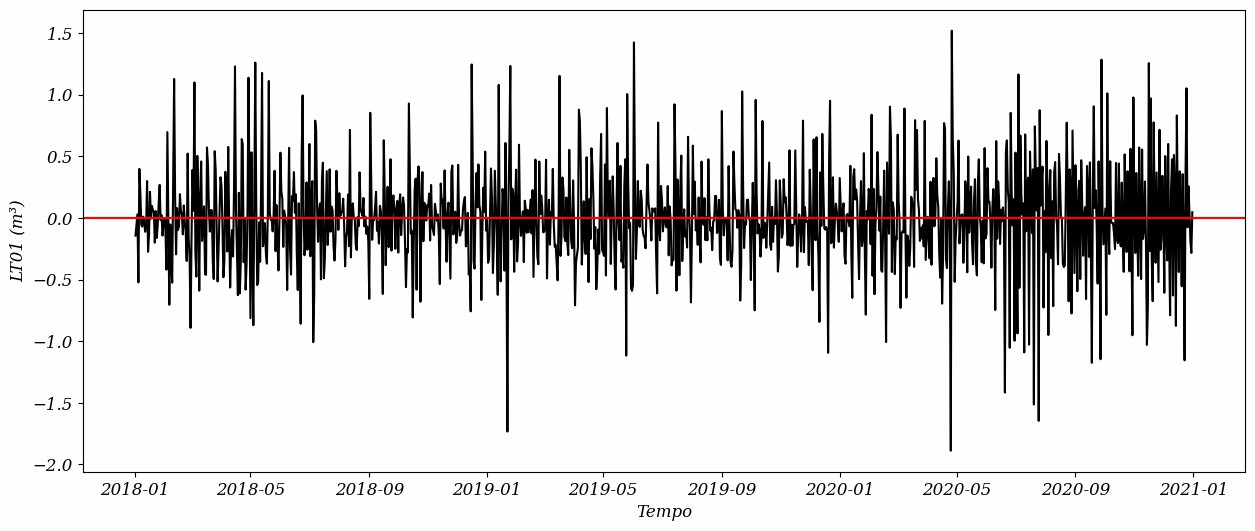
\includegraphics[width=0.9\linewidth]{Resultados/Figuras/ruido-branco}
	
	Fonte: Elaboração própria a partir de dados da SANEPAR (2018 a 2020)
\end{figure}

Na Figura \ref{fig:ruido-branco}, é possível observar uma série temporal que pode ser caracterizada como ruído branco. Uma série temporal é considerada ruído branco se suas variáveis forem independentes e distribuídas de forma idêntica, com média zero. Isso implica que todas as variáveis possuem a mesma variância ($\sigma^2$) e que cada valor não possui correlação com os demais valores da série.

Além disso, é importante destacar o comprimento dos zeros na variável prevista, o que conclui a etapa \ref{etp:3}.